% Метод погруженной границы.
\subsection{Метод погруженной границы с использованием фиктивных ячеек в трехмерной постановке}\label{sec:text_1_immersed_boundary_method}

При численном решении задач газовой динамики зачастую приходится сталкиваться с областями, обладающими сложной границей (это касается задач обтекания тел со сложной или изменяемой геометрией или расчета потоков внутри областей неправильной формы) \cite{Mahesh2003,Ye2020}.
Одним из наиболее ярких примеров проведения расчетов для областей со сложной геометрией является задача формирования ледяного нароста, для которой требуется постоянно пересчитывать аэродинамическое течение в условиях изменения геометрии обтекаемого тела из-за нарастания слоя льда \cite{Wright2015,BourgaultCote2017,Tong2016}.
Для таких областей построение согласованной расчетной сетки может быть крайне требовательной по ресурсам задачей (в некоторых случаях проведение расчетов для таких областей возможно только с использованием неструктурированных или гибридных сеток).
Альтернативой в данном случае является использование метода погруженной границы (immersed boundary method\label{term:immersed_boundary_method}, IBM\label{abbr:ibm}) \cite{Abalakin2018,Mori2008,Kim2004}.
Данный метод позволяет использовать для расчетов несогласованную сетку и даже простую декартову сетку \cite{Clarke1996}, что сильно упрощает и ускоряет проведение вычислений.
Применение метода погруженной границы позволяет проводить расчеты на простых структурированных сетках \cite{Farrashkhalvat2003,Rybakov2017}, что также упрощает имплементацию многопоточных вычислений и распараллеливание расчетных задач и балансировку их выполнения на большом количестве вычислительных узлов суперкомпьютерного кластера \cite{Savin2019,Giordano2019}.
Единственным тонким моментом метода является выполнение граничных условий на сложной границе, которое достигается путем модификации решаемой системы уравнений \cite{Fadlun2000}.
Можно выделить два основных подхода к разрешению граничных условий в методах погруженной границы, различающихся по способу выполнения расчетов на границе: задание граничных условий посредством внешних (источниковых) членов [15] и методы, использующие фиктивные (вспомогательные в расчетах) ячейки \cite{Tseng2003}.

Рассмотрим подробнее метод погруженной границы с использованием фиктивных ячеек \cite{Peter2016} на примере задачи обтекания тела со сложной геометрией.
Пусть в некоторой области пространства расположено тело, ограниченное сложной границей, представленной неструктурированной поверхностной расчетной сеткой.
В охватывающей тело области пространства строится объемная расчетная сетка, ячейки которой разделяются на следующие три основные класса: внешние, внутренние и граничные.
Внешними ячейками будем называть те ячейки, которые целиком лежат вне тела.
Внутренние ячейки лежат целиком внутри тела, все остальные ячейки пересекают границу тела и являются граничными.
В методе фиктивных ячеек из граничных ячеек выделяются ячейки, для которых меньшая часть объема находится вне тела, а большая - внутри тела.
Такие ячейки называются фиктивными.
Данное разделение является первичным и весьма приближенным, так как после коррекции некоторые внутренние ячейки могут быть также переведены в разряд фиктивных (в процессе проведения вычислений должно выполняться следующее требование: соседями внутренних ячеек не могут являться ни граничные, ни внешние ячейки).
На каждой итерации расчетов для фиктивных ячеек требуется выполнить аппроксимацию газодинамических величин (плотность, давление, вектор скорости), чтобы данные фиктивные ячейки могли быть использованы для определения потоков между ними и соседними с ними граничными и внешними ячейками \cite{Vinnikov2007}.
Таким образом, классификация ячеек объемной сетки является неотъемлемой частью метода погруженной границы.

Аппроксимация газодинамических параметров фиктивных ячеек выполняется на каждой итерации проведения расчетов, после для всех ячеек расчетной сетки кроме внутренних выполняется пересчет потоков между ячейками с использованием любого конечно-объемного метода. Обработка фиктивных ячеек является основной особенностью рассматриваемого метода, для вычисления газодинамических параметров фиктивных ячеек требуется использование аппроксимации скалярных и векторных величин по данным, взятым из близлежащих точек пространства и поверхности обтекаемого тела.

\subsubsection{Формулы аппроксимации скалярных и векторных величин в методе погруженной границы}

В данном разделе рассматриваются теоретические основы, которые используются при вычислении скалярных и векторных физических величин в фиктивных ячейках расчетной сетки.
Сначала рассмотрим формулу линейной аппроксимации скалярной величины по заданным четырем точкам в пространстве.
Пусть в пространстве определена скалярная величина $\phi = \phi(x, y, z)$ как функция от трех координат.
Пусть известно значение данной величины в четырех точках пространства: $\phi(x_0, y_0, z_0) = \phi_0$, $\phi(x_1, y_1, z_1) = \phi_1$, $\phi(x_2, y_2, z_2) = \phi_2$, $\phi(x_3, y_3, z_3) = \phi_3$.
Требуется выполнить линейную аппроксимацию данной величины, то есть найти представление вида $\phi(x, y, z) = a_0 + a_1x + a_2y + a_3z$, где коэффициенты $a_0$ , $a_1$, $a_2$, $a_3$ находятся по известным значениям в четырех точках.
Для двумерного случая задача описана в \cite{Tseng2003}, и в трехмерном варианте она выглядит аналогично.
Приведем подробное описание задачи для трехмерной постановки.
Для нахождения коэффициентов $a_0$, $a_1$, $a_2$, $a_3$ решается следующая система линейных уравнений:
\begin{equation}
	\left\{
		\begin{aligned}
			a_0 + a_1x_0 + a_2y_0 + a_3z_0 = \phi_0 \\
			a_0 + a_1x_1 + a_2y_1 + a_3z_1 = \phi_1 \\
			a_0 + a_1x_2 + a_2y_2 + a_3z_2 = \phi_2 \\
			a_0 + a_1x_3 + a_2y_3 + a_3z_3 = \phi_3
		\end{aligned}
	\right.
\end{equation}

Данная система уравнений может быть записана в матричной форме в следующем виде:
\begin{equation}
	B_{<0123>}a = \phi_{<0123>},
\end{equation}

где $\phi_{<0123>}$ -- это вектор-столбец $[\phi_0, \phi_1, \phi_2, \phi_3]^T$, $a$ -- вектор-столбец искомых коэффициентов $[a_0, a_1, a_2, a_3]^T$, а матрица $B_{<0123>}$ имеет вид
\begin{equation}\label{eqn:text_1_ibm_B}
	B_{<0123>} =
	\begin{bmatrix}
		1 & x_0 & y_0 & z_0 \\
		1 & x_1 & y_1 & z_1 \\
		1 & x_2 & y_2 & z_2 \\
		1 & x_3 & y_3 & z_3
	\end{bmatrix}
\end{equation}

Отсюда можно найти коэффициенты по формуле $a = B_{<0123>}^{-1}\phi_{<0123>}$.

Следующим шагом рассмотрим аппроксимацию все той жескалярной величины $\phi = \phi(x, y, z)$ с использованием граничного условия Неймана.
Только на этот раз пусть известно ее значение только в трех точках: $\phi(x_1, y_1, z_1) = \phi_1$, $\phi(x_2, y_2, z_2) = \phi_2$, $\phi(x_3, y_3, z_3) = \phi_3$.
Дополнительно в точке $(x_0, y_0, z_0)$ задано условие, соответствующее граничному условию Неймана:
\begin{equation}
	\frac{\partial{\phi}}{\partial{\overline{}_0}}(x_0, y_0, z_0) = \phi'_0
\end{equation}

где $\overline{e}_0$ -- некоторое направление (граничное условие Неймана задается как производная по нормали к поверхности обтекаемого тела).
При этом будем полагать, что $\overline{e}_0 = 1$.
Для заданной скалярной величины также требуется выполнить линейную аппроксимацию, то есть найти представление вида $\phi(x, y, z) = a_0 + a_1x + a_2y + a_3z$.
Для двумерного случая задача описана в \cite{Tseng2003}, приведем ее описание в трехмерном случае.

Пусть компоненты вектора направления $\overline{e}_0$ равны $e_{0,x}$, $e_{0,y}$, $e_{0,z}$ соответственно.
Граничное условие Неймана записывается в следующем виде:
\begin{equation}
	\frac{\partial{\phi}}{\partial{\overline{e}_0}}(x_0, y_0, z_0) = \frac{\partial{\phi}}{\partial{x}}e_{0,x} + \frac{\partial{\phi}}{\partial{y}}e_{0,y} + \frac{\partial{\phi}}{\partial{z}}e_{0,z} = \phi'_0
\end{equation}

Так как известен общий вид аппроксимации функции $\phi(x, y, z) = a_0 + a_1x + a_2y + a_3z$, то и ее частные производные можно выписать в явном виде: $\frac{\partial{\phi}}{\partial{x}} = a_1$, $\frac{\partial{\phi}}{\partial{y}} = a_2$, $\frac{\partial{\phi}}{\partial{z}} = a_3$.
Таким образом, получаем систему из четырех линейных уравнений:
\begin{equation}
	\left\{
		\begin{aligned}
			a_1e_{0,x} + a_2e_{0,y} + a_3e_{0,z} = \phi'_0 \\
			a_0 + a_1x_1 + a_2y_1 + a_3z_1 = \phi_1 \\
			a_0 + a_1x_2 + a_2y_2 + a_3z_2 = \phi_2 \\
			a_0 + a_1x_3 + a_2y_3 + a_3z_3 = \phi_3
		\end{aligned}
	\right.
\end{equation}

Данная система уравнений может быть записана в матричной форме в следующем виде:
\begin{equation}
	B_{<0'123>}a = \phi_{<0'123>},
\end{equation}

где $\phi_{<0'123>}$ -- это вектор-столбец $[\phi'_0, \phi_1, \phi_2, \phi_3]^T$, $a$ -- вектор-столбец искомых коэффициентов $[a_0, a_1, a_2, a_3]^T$, а матрица $B_{<0'123>}$ имеет вид
\begin{equation}\label{eqn:text_1_ibm_B1}
	B_{<0'123>} =
	\begin{bmatrix}
		0 & e_{0,x} & e_{0,y} & e_{0,z} \\
		1 & x_1 & y_1 & z_1 \\
		1 & x_2 & y_2 & z_2 \\
		1 & x_3 & y_3 & z_3
	\end{bmatrix}
\end{equation}

Отсюда получим выражение для коэффициентов линейной аппроксимации $a = B_{<0'123>}^{-1}\phi_{<0'123>}$.

После рассмотрения вопросов, связанных со скалярными величинами, перейдем к векторным физическим величинам.
Для двумерного случая вопрос рассмотрен в \cite{Vinnikov2007}, однако в трехмерном случае задача несколько сложнее.
При решении задач обтекания тел со сложной геометрией важнейшим вопросом является вычисление значения скорости в фиктивных ячейках, а скорость является векторной величиной.
Итак, рассмотрим векторную величину $\overline{v} = [v_x, v_y, v_z] = [v_x(x, y, z), v_y(x, y, z), v_z(x, y, z)]$, которая задана в трехмерном пространстве как функция от трех координат.
Пусть известны ее значения в трех точках:
\begin{equation}
	\begin{aligned}
		\overline{v}(x_1, y_1, z_1) = \overline{v}_1 = [v_{1,x}, v_{1,y}, v_{1,z}] \\
		\overline{v}(x_2, y_2, z_2) = \overline{v}_2 = [v_{2,x}, v_{2,y}, v_{2,z}] \\
		\overline{v}(x_3, y_3, z_3) = \overline{v}_3 = [v_{3,x}, v_{3,y}, v_{3,z}]
	\end{aligned}
\end{equation}

Дополнительно в точке $(x_0, y_0, z_0)$ задано следующее условие: проекция вектора $\overline{v}_0 = \overline{v}(x_0, y_0, z_0)$ на направление $\overline{e}_0$ равна нулю, а производная составляющей, перпендикулярной данному направлению, по этому направлению также равна нулю.
То есть
\begin{equation}
	\left\{
		\begin{aligned}
			\overline{v}_0 = \overline{v}_0^n + \overline{v}_0^{\tau} \\
			\overline{v}_0^n \parallel \overline{e}_0 \\
			\overline{v}_0^{\tau} \perp \overline{e}_0 \\
			|\overline{e}_0| = 1 \\
			|\overline{v}_0^n| = 0 \\
			\frac{\partial{|\overline{v}^{\tau}|}}{\partial{\overline{e}_0}}(x_0, y_0, z_0) = 0 
		\end{aligned}
	\right.
\end{equation}

Требуется определить значение векторной величины в некоторой точке $(x_G, y_G, z_G)$, то есть $\overline{v}_G = \overline{v}(x_G, y_G, z_G)$.
При этом под направлением $\overline{e}_0$ будем подразумевать некоторую нормаль к поверхности обтекаемого тела, для которого выполняется расчет.
Тогда логично называть составляющие вектора $\overline{v}_0^n$ и $\overline{v}_0^{\tau}$ нормальной и тангенциальной составляющими вектора $\overline{v}_0$ соответственно.
Сначала запишем условие равенства нулю нормальной составляющей вектора $\overline{v}_0$, выражающееся в равенстве нулю скаляр-
ного произведения $(\overline{v}_0, \overline{e}_0)$. 
Распишем данное произведение покомпонентно:
\begin{equation}
	v_{0,x}e_{0,x} + v_{0,y}e_{0,y} + v_{0,z}e_{0,z} = 0
\end{equation}

Значения $v_{0,x}$, $v_{0,y}$, $v_{0,z}$ нам не известны, поэтому выразим их с помощью линейной интерполяции скалярной величины через точки $P_1 = (x_1, y_1, z_1)$, $P_2 = (x_2, y_2, z_2)$, $P_3 = (x_3, y_3, z_3)$, $P_G = (x_G, y_G, z_G)$:
\begin{equation}
	\left\{
		\begin{aligned}
			v_{0,x} = [1, x_0, y_0, z_0] B_{<G123>}^{-1} v_{<G123>,x} \\
			v_{0,y} = [1, x_0, y_0, z_0] B_{<G123>}^{-1} v_{<G123>,y} \\
			v_{0,z} = [1, x_0, y_0, z_0] B_{<G123>}^{-1} v_{<G123>,z}
		\end{aligned}
	\right.
\end{equation}

Подставляя полученные соотношения для $v_{0,x}$, $v_{0,y}$, $v_{0,z}$ в выражение скалярного произведения $(\overline{v}_0, \overline{e}_0) = 0$, получим:
\begin{equation}
	[1, x_0, y_0, z_0] B_{<G123>}^{-1}
	\left(
		\begin{bmatrix}
			v_{G,x} \\
			v_{1,x} \\
			v_{2,x} \\
			v_{3,x}
		\end{bmatrix} e_{0,x} +
		\begin{bmatrix}
			v_{G,y} \\
			v_{1,y} \\
			v_{2,y} \\
			v_{3,y}
		\end{bmatrix} e_{0,y} +
		\begin{bmatrix}
			v_{G,z} \\
			v_{1,z} \\
			v_{2,z} \\
			v_{3,z}
		\end{bmatrix} e_{0,z}
	\right) = 0
\end{equation}

Введем обозначения $[d_G, d_1, d_2, d_3] = [1, x_0, y_0, z_0] B_{<G123>}^{-1}$, тогда уравнение может быть переписано в следующем виде:
\begin{equation}
	d_G(v_{G,x}e_{0,x} + v_{G,y}e_{0,y} + v_{G,z}e_{0,z}) + d_1(\overline{v}_1, \overline{e}_0) + d_2(\overline{v}_2, \overline{e}_0) + d_3(\overline{v}_3, \overline{e}_0) = 0
\end{equation}

Перепишем это уравнение в виде
\begin{equation}
	v_{G,x}e_{0,x} + v_{G,y}e_{0,y} + v_{G,z}e_{0,z} = Q
\end{equation}

где значение $Q$ может быть вычислено явно следующим образом:
\begin{equation}
	Q = -\frac{d_1(\overline{v}_1, \overline{e}_0) + d_2(\overline{v}_2, \overline{e}_0) + d_3(\overline{v}_3, \overline{e}_0)}{d_G}
\end{equation}

Условие на тангенциальную составляющую $\overline{v}_0^{\tau}$ не будем записывать в явном виде.
Вместо этого будем работать с проекциями вектора $\overline{v}_0$ на векторы, лежащие в плоскости, перпендикулярной вектору $\overline{e}_0$.
Так как компоненты вектора $\overline{e}_0$ известны, то можно без труда найти векторы, перпендикулярные ему.
Это будут, например, следующие векторы: $\overline{f}_1 = [-e_{0,y}, e_{0,x}, 0]$, $\overline{f}_2 = [-e_{0,z}, 0, e_{0,x}]$, $\overline{f}_3 = [0, -e_{0,z}, e_{0,y}]$.

Далее запишем выражения для линейной аппроксимации величин $(\overline{f}_1, \overline{v}_G)$, $(\overline{f}_2, \overline{v}_G)$, $(\overline{f}_3, \overline{v}_G)$ через точки $P_0$ , $P_1$ , $P_2$ , $P_3$ с учетом граничного условия Неймана:
\begin{equation}
	\left\{
		\begin{aligned}
			-v_{G,x}e_{0,y} + v_{G,y}e_{0,x} = [1,x_G,y_G,z_G] B_{<0'123>}^{-1}
			\begin{bmatrix}
				0 \\
				-v_{1,x}e_{0,y} + v_{1,y}e_{0,x} \\
				-v_{2,x}e_{0,y} + v_{2,y}e_{0,x} \\
				-v_{3,x}e_{0,y} + v_{3,y}e_{0,x}
			\end{bmatrix} \\
			-v_{G,x}e_{0,z} + v_{G,z}e_{0,x} = [1,x_G,y_G,z_G] B_{<0'123>}^{-1}
			\begin{bmatrix}
				0 \\
				-v_{1,x}e_{0,z} + v_{1,z}e_{0,x} \\
				-v_{2,x}e_{0,z} + v_{2,z}e_{0,x} \\
				-v_{3,x}e_{0,z} + v_{3,z}e_{0,x}
			\end{bmatrix} \\
			-v_{G,y}e_{0,z} + v_{G,z}e_{0,y} = [1,x_G,y_G,z_G] B_{<0'123>}^{-1}
			\begin{bmatrix}
				0 \\
				-v_{1,y}e_{0,z} + v_{1,z}e_{0,y} \\
				-v_{2,y}e_{0,z} + v_{2,z}e_{0,y} \\
				-v_{3,y}e_{0,z} + v_{3,z}e_{0,y}
			\end{bmatrix}
		\end{aligned}
	\right.
\end{equation}

В приведенной выше системе уравнений правые части могут быть непосредственно вычислены, обозначим их $T_{xy}$ , $T_{xz}$ и $T_{yz}$ соответственно и добавим в систему уравнение для выражения $(\overline{v}_G, \overline{e}_0)$.
Получим следующую систему:
\begin{equation}
	\left\{
		\begin{aligned}
			v_{G,x}e_{0,x} + v_{G,y}e_{0,y} + v_{G,z}e_{0,z} = Q \\
			-v_{G,x}e_{0,y} + v_{G,y}e_{0,x} = T_{xy} \\
			-v_{G,x}e_{0,z} + v_{G,z}e_{0,x} = T_{xz} \\
			-v_{G,y}e_{0,z} + v_{G,z}e_{0,y} = T_{yz}			
		\end{aligned}
	\right.
\end{equation}

В матричной форме данная система может быть записана следующим образом:
\begin{equation}
	\begin{bmatrix}
		e_{0,x} & e_{0,y} & e_{0,z} \\
		-e_{0,y} & e_{0,x} & 0 \\
		-e_{0,z} & 0 & e_{0,x} \\
		0 & -e_{0,z} & e_{0,y}
	\end{bmatrix}
	\begin{bmatrix}
		v_{G,x} \\
		v_{G,y} \\
		v_{G,z}
	\end{bmatrix} =
	\begin{bmatrix}
		Q \\
		T_{xy} \\
		T_{xz} \\
		T_{yz}
	\end{bmatrix}			
\end{equation}

В приведенной системе 4 уравнения и 3 неизвестных, поэтому одно из трех последних уравнений избыточно.
Заметим, что если две компоненты вектора $\overline{e}_0$ равны нулю, то один из векторов $\overline{f}_1$, $\overline{f}_2$ , $\overline{f}_3$ вырождается в нулевой вектор.
Если же только одна компонента вектора $\overline{e}_0$ равна нулю, то два из векторов $\overline{f}_1$, $\overline{f}_2$ , $\overline{f}_3$ становятся коллинеарными.
\begin{equation}
	\left\{
		\begin{aligned}
			e_{0,x} = 0, e_{0,y} = 0, e_{0,z} \ne 0 \implies \overline{f}_1 = \overline{0} \\
			e_{0,x} = 0, e_{0,z} = 0, e_{0,y} \ne 0 \implies \overline{f}_2 = \overline{0} \\
			e_{0,y} = 0, e_{0,z} = 0, e_{0,x} \ne 0 \implies \overline{f}_3 = \overline{0} \\
			e_{0,x} = 0, e_{0,y} \ne 0, e_{0,z} \ne 0 \implies \overline{f}_1 \parallel \overline{f}_2 \\
			e_{0,y} = 0, e_{0,x} \ne 0, e_{0,z} \ne 0 \implies \overline{f}_1 \parallel \overline{f}_3 \\
			e_{0,z} = 0, e_{0,x} \ne 0, e_{0,y} \ne 0 \implies \overline{f}_2 \parallel \overline{f}_3
		\end{aligned}
	\right.
\end{equation}

Из результирующей системы уравнений будем исключать то уравнение, в которое входит наименьшая по модулю компонента вектора $\overline{e}_0$.
Запишем это явно.

Если наименьшей по модулю компонентой вектора $\overline{e}_0$ является $e_{0,x}$ то
\begin{equation}
	[v_{G,x}, v_{G,y}, v_{G,z}]^T =
	\begin{bmatrix}
		e_{0,x} & e_{0,y} & e_{0,z} \\
		-e_{0,y} & e_{0,x} & 0 \\
		0 & -e_{0,z} & e_{0,y}
	\end{bmatrix}
	[Q, T_{xy}, T_{yz}]^T = E^x[Q, T_{xy}, T_{yz}]^T
\end{equation}

Если наименьшая по модулю компонента вектора $\overline{e}_0$ это $e_{0,y}$ или $e_{0,z}$ то
\begin{equation}
	[v_{G,x}, v_{G,y}, v_{G,z}]^T =
	\begin{bmatrix}
		e_{0,x} & e_{0,y} & e_{0,z} \\
		-e_{0,y} & e_{0,x} & 0 \\
		-e_{0,z} & 0 & e_{0,x}
	\end{bmatrix}
	[Q, T_{xy}, T_{xz}]^T = E^{yz}[Q, T_{xy}, T_{xz}]^T
\end{equation}

Полученные в данном разделе формулы были использованы для аппроксимации скалярных (плотность, давление) и векторных (скорость) физических величин в фиктивных ячейках при реализации метода погруженной границы для обтекания тел со сложной геометрией.

\subsubsection{Реализация метода погруженной границы}\label{sec:text_1_immersed_boundary_method_realization}

Первым шагом проведения вычислений с использованием метода погруженной границы является выполнение классификации ячеек объемной сетки.
На рис.~\ref{fig:text_1_immersed_boundary_method_1} показана первичная классификация ячеек для двумерного случая.

\begin{figure}[ht]
	\centering
		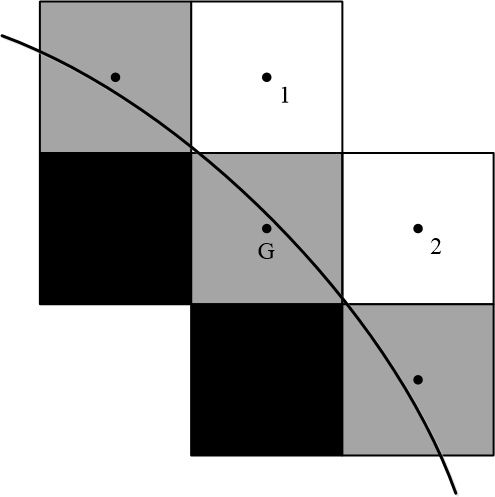
\includegraphics[width=0.30\textwidth]{./pics/text_1_immersed_boundary_method/ghost_cells_2d.png}
	\caption{Двумерная иллюстрация разделения ячеек расчетной сетки на внешние, граничные и внутренние.}
	\label{fig:text_1_immersed_boundary_method_1}
\end{figure}

На этапе первичной классификации решается задача нахождения пересечения поверхности обтекаемого тела с ячейками расчетной сетки \cite{Rybakov2019VecInt} (см. рис.~\ref{fig:text_1_mesh_intersect_contour}).

\begin{figure}[ht]
	\centering
	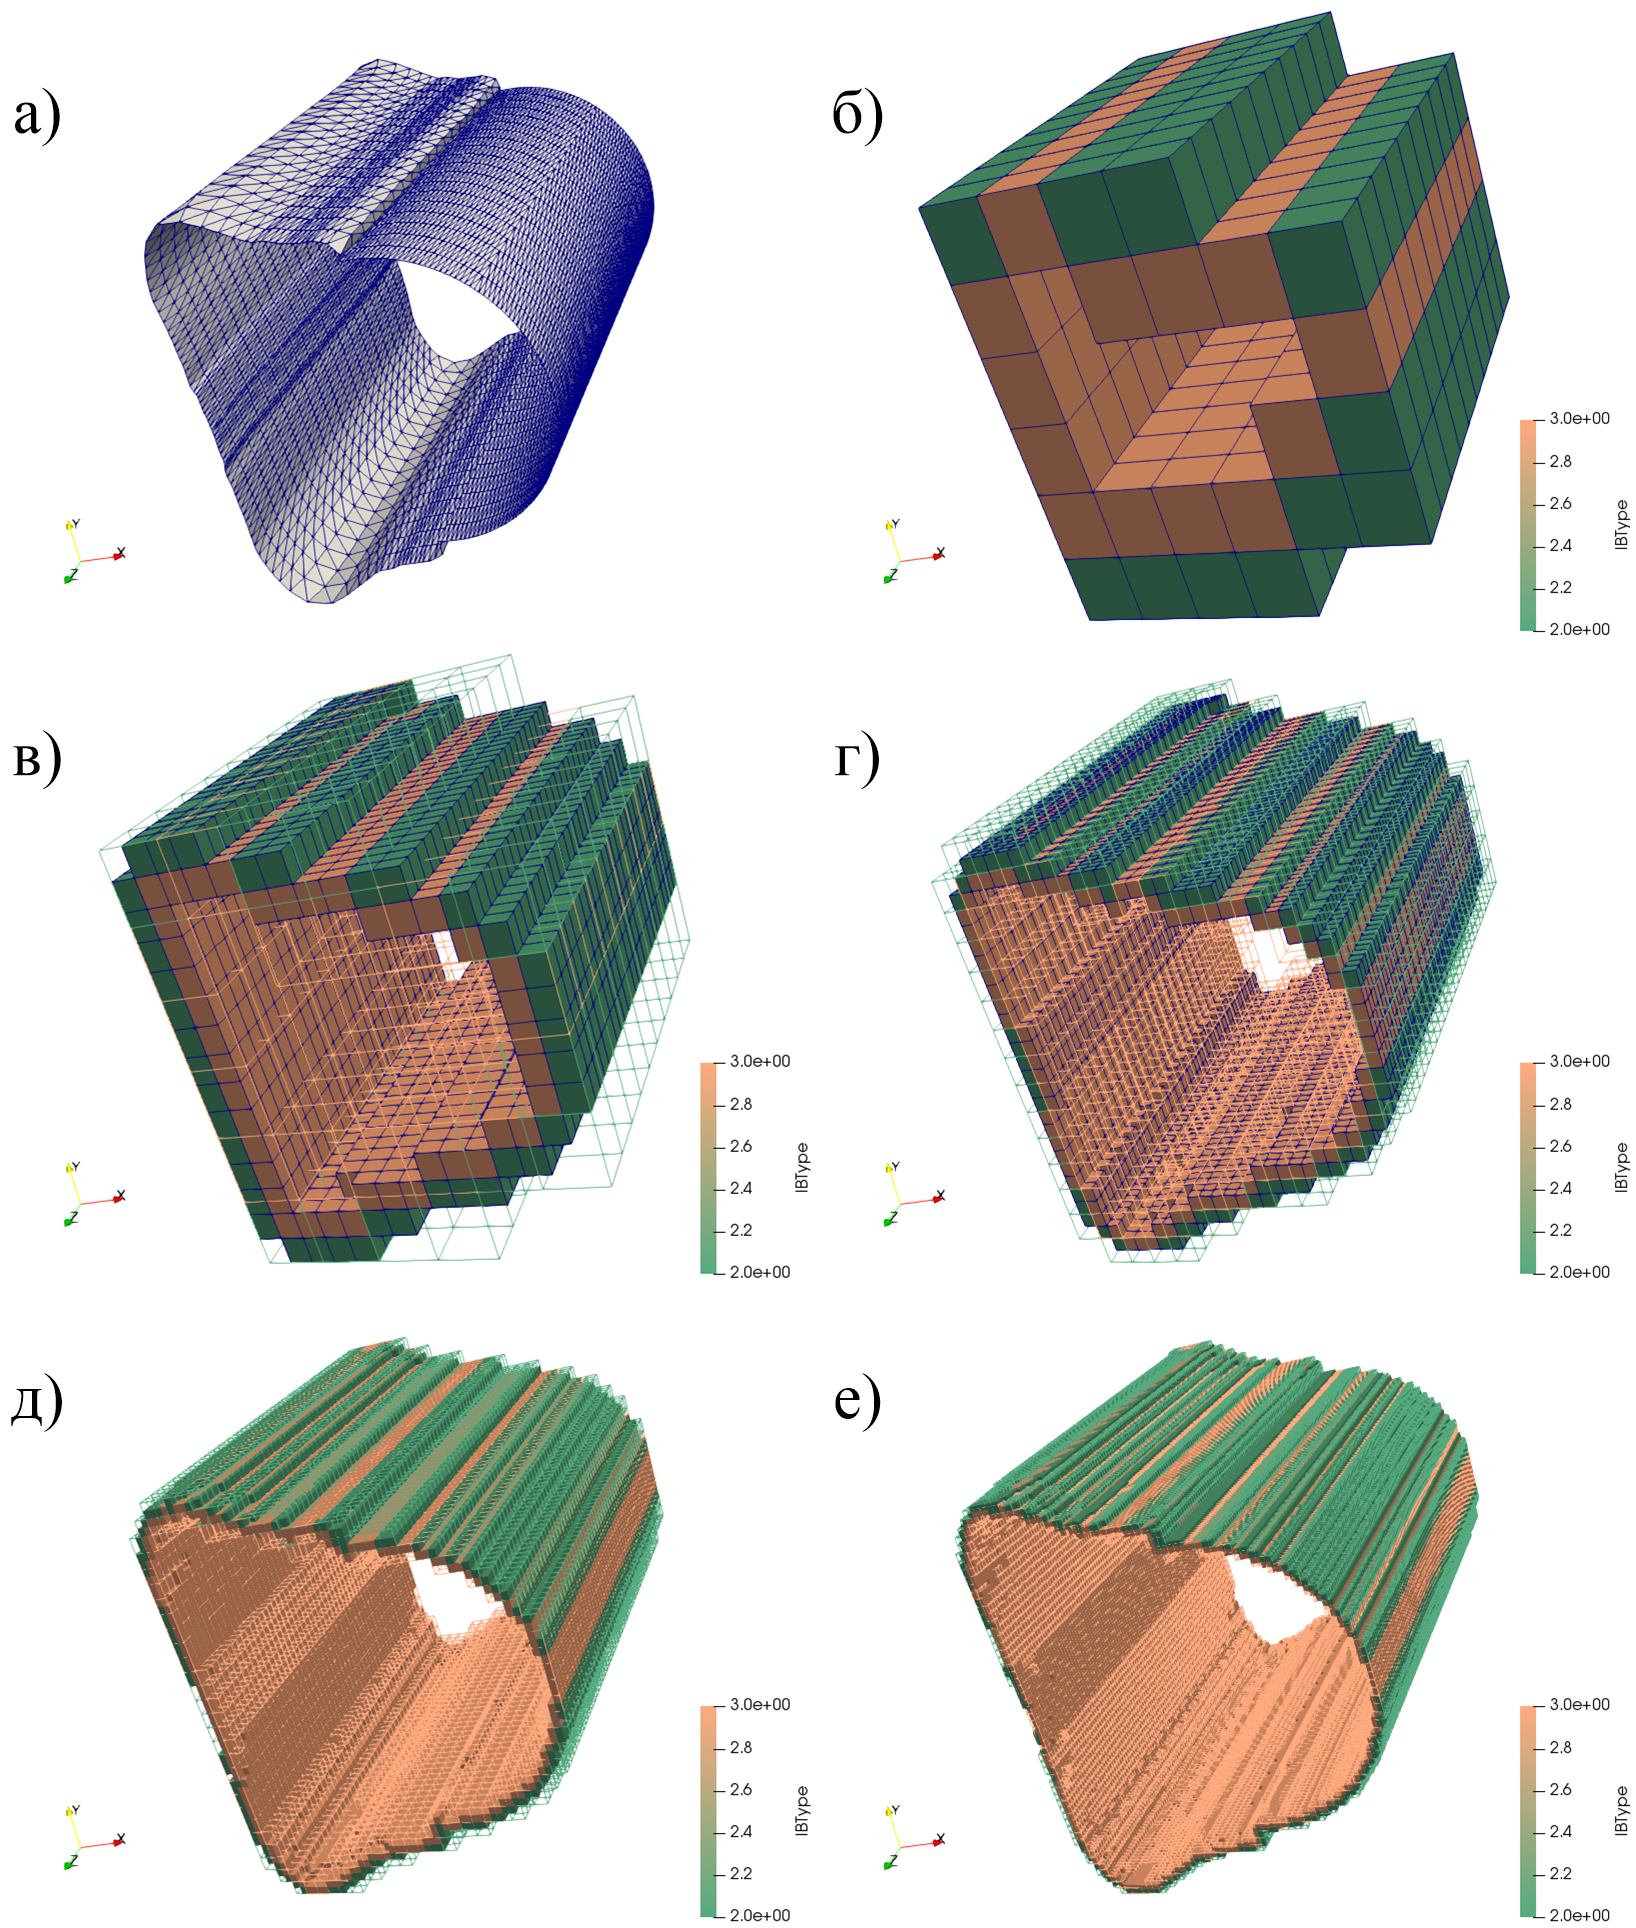
\includegraphics[width=0.6\textwidth]{./pics/text_4_mesh_intersect/contour.png}
	\caption{Иллюстрация пересечения поверхностной сетки и объемных сеток с разным количеством ячеек. На рисунках цветами обозначены только граничные и фиктивные ячейки объемной сетки (граничные -- зеленые, фиктивные -- бежевые). а) Исходная геометрия поверхностной сетки. б) Размер объемной сетки $10 \times 10 \times 10$. в) Размер объемной сетки $25 \times 25 \times 25$. г) Размер объемной сетки $50 \times 50 \times 50$. д) Размер объемной сетки $100 \times 100 \times 100$. е) Размер объемной сетки $150 \times 150 \times 150$.}
	\label{fig:text_1_mesh_intersect_contour}
\end{figure}

Если пересечение зафиксировано, то ячейка получает статус граничной ячейки (показа на рис.~\ref{fig:text_1_immersed_boundary_method_1} серым цветом).
Далее выполняется обход ячеек объемной сетки, в ходе которого все оставшиеся ячейки делятся на внешние (целиком находятся вне обтекаемого тела) и на внутренние (целиком находятся внутри обтекаемого тела).
На втором этапе классификации ячеек из множества граничных ячеек выделяются фиктивные ячейки - ячейки, большая часть объема которых находится внутри обтекаемого тела.
Наконец третий этап классификации ячеек предусматривает коррекцию, в ходе которой внутренние ячейки, имеющие в качестве соседей граничные ячейки, получат статут фиктивных.
Таким образом, обеспечивается выполнение требования, что внутренние ячейки не могут контактировать по грани с граничными и, тем более, с внешними ячейками.

На каждой итерации выполнения расчетов для каждой фиктивной ячейки должны быть пересчитаны газодинамические величины на основании данных близлежащих граничных или внешних ячеек (рассматриваются точки, являющиеся центрами таких ячеек), а также точки поверхности обтекаемого тела для аппроксимации граничного условия (для каждой фиктивной ячейки используется ближайшая к ней точка поверхности).
Данные точки могут выбираться в некоторой степени произвольно, однако нужно контролировать, чтобы при проведении аппроксимации параметров фиктивных ячеек по формулам, приведенным в предыдущем разделе, никакие матрицы не оказались вырожденными.
Набор точек, по которым производится аппроксимация данных для фиктивной ячейки, будем называть шаблоном.
Для каждой ячейки существует огромное количество шаблонов даже при использовании простой декартовой расчетной сетки (например, в трехмерном случае общее количество шаблонов для фиктивной ячейки, превышает 1000 штук, даже если рассматривать только ближайших соседей).
При использовании же адаптивных локально-измельчающихся сеток \cite{Wackers2011,Zhou2014,Plas2015} количество шаблонов резко возрастает, а для таких сеток применение метода погруженной границы представляет особенный интерес.
Многие из этих шаблонов можно не рассматривать изначально (например это шаблоны, в которые попадают внутренние ячейки или другие фиктивные ячейки), другие шаблоны нужно отсеивать по специальным критериям (например, шаблон, в котором точка поверхности обтекаемого тела лежит слишком близко к какой-нибудь другой точке шаблона).

Конечно, наибольший интерес представляет аппроксимация векторных величин, а именно аппроксимация вектора скорости в фиктивной ячейке.
Поэтому вопрос аппроксимации скалярных характеристик фиктивных ячеек мы опустим.
На рис.~\ref{fig:text_1_immersed_boundary_method_2} приведена иллюстрация выполнения аппроксимации вектора скорости для двумерного случая (трехмерный случай обрабатывается аналогично).
Фиктивная ячейка, центр которой обозначен буквой $G$, большей частью находится внутри обтекаемого тела.
Для выполнения аппроксимации вектора скорости в данной ячейки в качестве шаблона выбраны две соседние граничные ячейки (центры которых обозначены цифрами $1$ и $2$), а также ближайшая к $G$ точка поверхности обтекаемого тела.
Данный шаблон (точки $0$, $1$, $2$) вполне подходит для выполнения аппроксимации, так как никакие две точки в нем не совпадают, а также перечисленные точки не лежат на одной прямой, в дополнение направление нормали, проведенной из точки $0$, не параллельно отрезку, соединяющему точки $1$ и $2$.

\begin{figure}[ht]
	\centering
		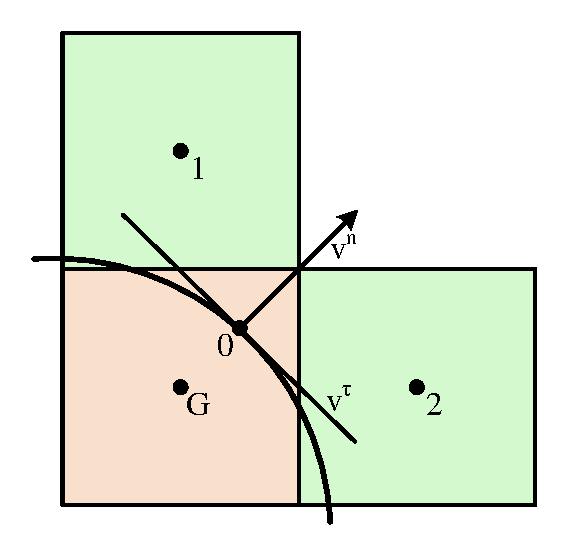
\includegraphics[width=0.50\textwidth]{./pics/text_1_immersed_boundary_method/3_points_lin_appr_velocity_2d.pdf}
	\caption{Двумерная иллюстрация аппроксимации скорости в фиктивной ячейке}
	\label{fig:text_1_immersed_boundary_method_2}
\end{figure}

Для верификации описанного метода погруженной границы (даже скорее самих формул аппроксимации газодинамических параметров фиктивных ячеек с использованием приближения граничных условий) была рассмотрена тестовая задача обтекания цилиндра свободным потоком.
Вокруг цилиндра была обстроена декартова объемная расчетная сетка с кубическими ячейками, выполнена их классификация, как это показано на рис.~\ref{fig:text_1_immersed_boundary_method_3} (на данном рисунке синим цветом показаны внешние ячейки, светло-синим цветом -- граничные, красным -- фиктивные, внутренние ячейки на рисунке проигнорированы).

\begin{figure}[ht]
	\centering
		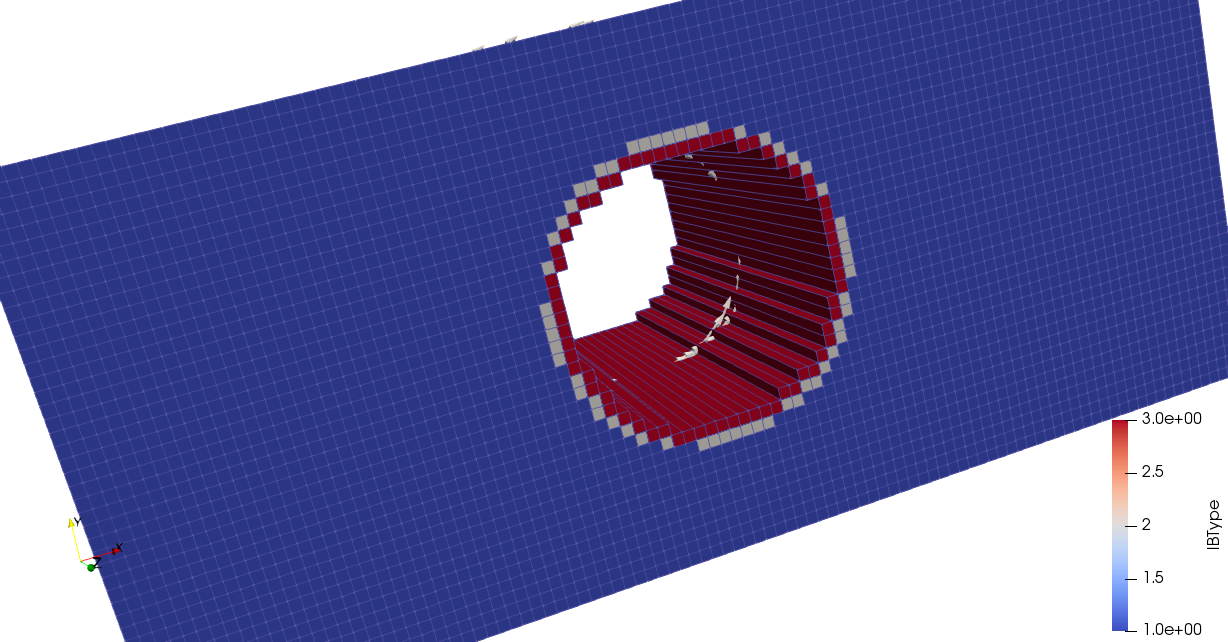
\includegraphics[width=0.80\textwidth]{./pics/text_1_immersed_boundary_method/3d_mesh.png}
	\caption{Разбиение расчетной области на внешние, граничные и фиктивные ячейки в задаче обтекания
цилиндра}
	\label{fig:text_1_immersed_boundary_method_3}
\end{figure}

В ходе выполнения расчетов решалась обычная нестационарная система уравнений Эйлера, описывающая трехмерное течение идеального газа. Для решения использовалась противопотоковая схема Steger-Warming с расщеплением потока \cite{Smirnova2018}.
В ходе выполнения расчетов получена качественная картина формирования поля скоростей с учетом обтекания цилиндра, представленная на рис.~\ref{fig:text_1_immersed_boundary_method_4}.

\begin{figure}[ht]
	\centering
		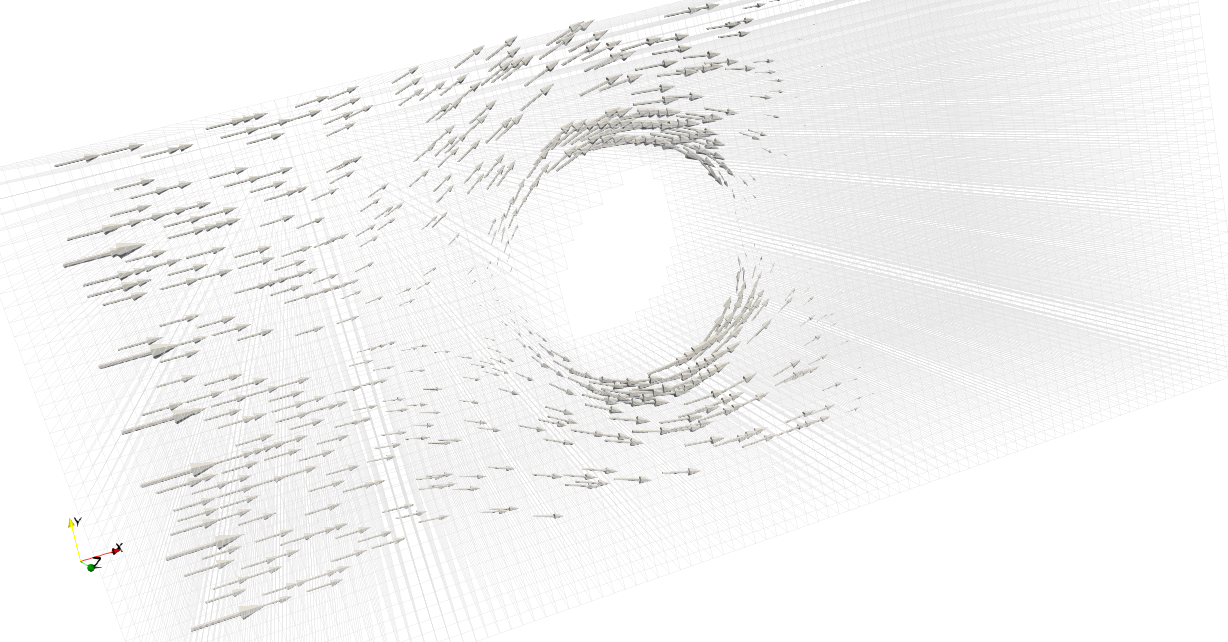
\includegraphics[width=0.80\textwidth]{./pics/text_1_immersed_boundary_method/velocity_field.png}
	\caption{Формирование поля скоростей в задаче обтекания цилиндра}
	\label{fig:text_1_immersed_boundary_method_4}
\end{figure}